\section{Auswertung}
\label{sec:Auswertung}

Zunächst wird die Wagengeschwindigkeit bei den zehn verschiedenen Gangeinstellungen des Wagens bestimmt.
Die Weglänge wird mithilfe eines Maßbandes zu
\begin{align*}
  s = \SI{43.8 +- 0.1}{\centi\metre}
\end{align*}
bestimmt.
Der jeweilige nominelle Wert für $t$ wird aus dem Mittelwert der fünf Einzelmessungen bestimmt.
Der Mittelwert berechnet sich dabei mithilfe der Formel
\begin{equation}
 \bar{x} = \frac{1}{n} \sum_{i=1}^n x_i.
\end{equation}
Der Fehler der Zeit wird mittels der Standardabweichung aus den fünf Einzelwerten bestimmt.
Die Standardabweichung berechnet sich dabei nach
\begin{equation}
  s = \sqrt{\frac{1}{n+1} \sum_{i=1}^n (x_i - \bar{x}) }.
\end{equation}
Unter der Annahme einer linearen Bewegung wird die Geschwindigkeit nun mit dem Weg-Zeit-Gesetz berechnet.
Für die Fehlerrechnung wird bei der vorliegenden Rechnung und bei allen folgenden Rechnungen das Gaußsche Fehlerfortpflanzungsgesetz
\begin{equation}
\increment{f} = \sqrt{\Bigl(\frac{\partial f}{\partial x_1}\increment{x_1}\Bigr)^2 + \Bigl(\frac{\partial f}{\partial x_2}\increment{x_2}\Bigr)^2 + \dotsc + \Bigl(\frac{\partial f}{\partial x_n}\increment{x_n}\Bigr)^2}
\end{equation}
für eine Funktion $f(x_1,x_2, \dotsc ,x_n)$, bei der die Größen $x_1, x_2, \dotsc , x_n$ voneinander unabhängig sind, verwendet.
Es ergeben sich hieraus die in Tabelle \ref{tab:Geschwindigkeiten} angegebenen Werte.

\begin{table}[H]
  \centering
  \caption{Wagengeschwindigkeiten}
  \label{tab:Geschwindigkeiten}
  \sisetup{table-format=1.2}
  \begin{tabular}{c c c}
    \toprule
    {$\text{Gang}$} & {$v [\si{\centi\metre\per\second}]$} & {$\increment v [\si{\centi\metre\per\second}]$}\\
    \midrule
    \input{build/geschwtabelle.tex}
    \bottomrule
  \end{tabular}
\end{table}



\begin{align*}
  \lambda_0 &= \input{build/wl.tex}
\end{align*}



\begin{align*}
  c &= \input{build/c.tex}
\end{align*}

\begin{align*}
  \frac{1}{\lambda_0} &= \input{build/einsdurchwl.tex}
\end{align*}








%\begin{figure}
%  \centering
%  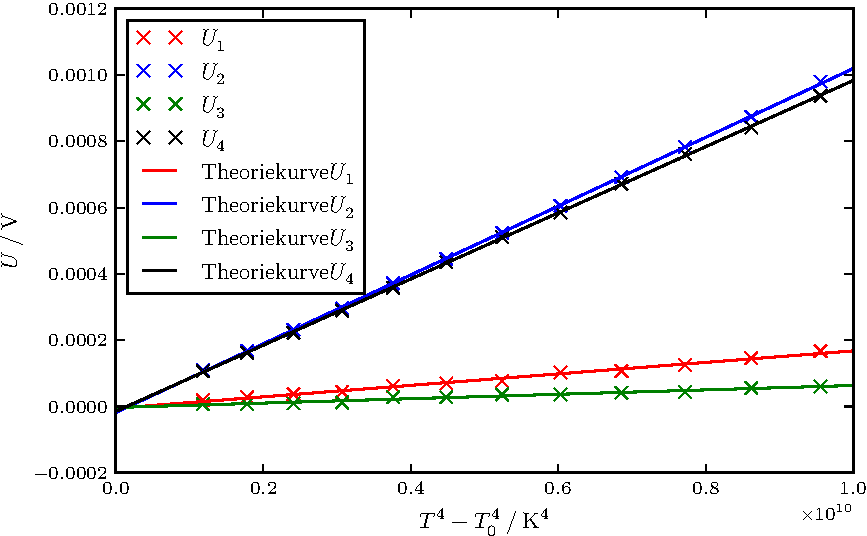
\includegraphics{plot.pdf}
%  \caption{Plot.}
%  \label{fig:plot}
%\end{figure}
%
%\begin{table}
%  \centering
%  \caption{Beispieltabelle}
%  \label{tab:tabelle_beispiel}
%  \sisetup{table-format=1.2}
%  \begin{tabular}{c c}
%    \toprule
%    {$a [\si{\second}]$} & {$b [\si{\kelvin}]$}\\
%    \midrule
%    1.0000  & 11.00 \\
2.0000  & 12.00 \\
3.0000  & 13.00 \\
4.0000  & 14.00 \\
5.0000  & 15.00 \\
6.0000  & 16.00 \\
7.0000  & 17.00 \\
8.0000  & 18.00 \\
9.0000  & 19.00 \\
10.0000 & 20.00 \\

%    \bottomrule
%  \end{tabular}
%\end{table}
%
%Es ergibt sich
%\begin{align}
%  a &= (0 \pm 0) ~ \si{\joule\per\kelvin\per\gram}
 \\
%\end{align}
